\documentclass{article}%
\usepackage[T1]{fontenc}%
\usepackage[utf8]{inputenc}%
\usepackage{lmodern}%
\usepackage{textcomp}%
\usepackage{lastpage}%
\usepackage{geometry}%
\geometry{margin=0.5in}%
\usepackage{graphicx}%
%
\title{Report on Weather Australia dataset}%
\author{Auto2Class}%
%
\begin{document}%
\normalsize%
\maketitle%
\newpage%
\tableofcontents%
\newpage%
\section{Exploratory Data Analysis Part}%
\label{sec:ExploratoryDataAnalysisPart}%
\subsection{DataTypes and Non{-}Null Count}%
\label{subsec:DataTypesandNon{-}NullCount}%


\begin{table}[h!]%
\caption{Dataset Columns Information}%
\vspace{0.2cm}%
\centering%
\begin{tabular}{|c|c|c|}%
\hline%
Column&Non{-}Null Count&Dtype\\%
\hline%
Date&145460&object\\%
Location&145460&object\\%
MinTemp&143975&float64\\%
MaxTemp&144199&float64\\%
Rainfall&142199&float64\\%
Evaporation&82670&float64\\%
Sunshine&75625&float64\\%
WindGustDir&135134&object\\%
WindGustSpeed&135197&float64\\%
WindDir9am&134894&object\\%
WindDir3pm&141232&object\\%
WindSpeed9am&143693&float64\\%
WindSpeed3pm&142398&float64\\%
Humidity9am&142806&float64\\%
Humidity3pm&140953&float64\\%
Pressure9am&130395&float64\\%
Pressure3pm&130432&float64\\%
Cloud9am&89572&float64\\%
Cloud3pm&86102&float64\\%
Temp9am&143693&float64\\%
Temp3pm&141851&float64\\%
RainToday&142199&object\\%
RainTomorrow&142193&object\\%
\hline%
\end{tabular}%
\end{table}

%
\newpage%
\subsection{Descriptive Statistics}%
\label{subsec:DescriptiveStatistics}%


\begin{table}[h!]%
\caption{Dataset Descriptive Statistics}%
\vspace{0.2cm}%
\centering%
\begin{tabular}{|c|c|c|c|c|c|c|c|c|}%
\hline%
Statistic&count&mean&std&min&25\%&50\%&75\%&max\\%
\hline%
MinTemp&143975.0&12.19&6.4&{-}8.5&7.6&12.0&16.9&33.9\\%
MaxTemp&144199.0&23.22&7.12&{-}4.8&17.9&22.6&28.2&48.1\\%
Rainfall&142199.0&2.36&8.48&0.0&0.0&0.0&0.8&371.0\\%
Evaporation&82670.0&5.47&4.19&0.0&2.6&4.8&7.4&145.0\\%
Sunshine&75625.0&7.61&3.79&0.0&4.8&8.4&10.6&14.5\\%
WindGustSpeed&135197.0&40.04&13.61&6.0&31.0&39.0&48.0&135.0\\%
WindSpeed9am&143693.0&14.04&8.92&0.0&7.0&13.0&19.0&130.0\\%
WindSpeed3pm&142398.0&18.66&8.81&0.0&13.0&19.0&24.0&87.0\\%
Humidity9am&142806.0&68.88&19.03&0.0&57.0&70.0&83.0&100.0\\%
Humidity3pm&140953.0&51.54&20.8&0.0&37.0&52.0&66.0&100.0\\%
Pressure9am&130395.0&1017.65&7.11&980.5&1012.9&1017.6&1022.4&1041.0\\%
Pressure3pm&130432.0&1015.26&7.04&977.1&1010.4&1015.2&1020.0&1039.6\\%
Cloud9am&89572.0&4.45&2.89&0.0&1.0&5.0&7.0&9.0\\%
Cloud3pm&86102.0&4.51&2.72&0.0&2.0&5.0&7.0&9.0\\%
Temp9am&143693.0&16.99&6.49&{-}7.2&12.3&16.7&21.6&40.2\\%
Temp3pm&141851.0&21.68&6.94&{-}5.4&16.6&21.1&26.4&46.7\\%
\hline%
\end{tabular}%
\end{table}

%
\newpage%
\subsection{Histograms of Numerical columns}%
\label{subsec:HistogramsofNumericalcolumns}%


\begin{figure}[h!]%
\centering%
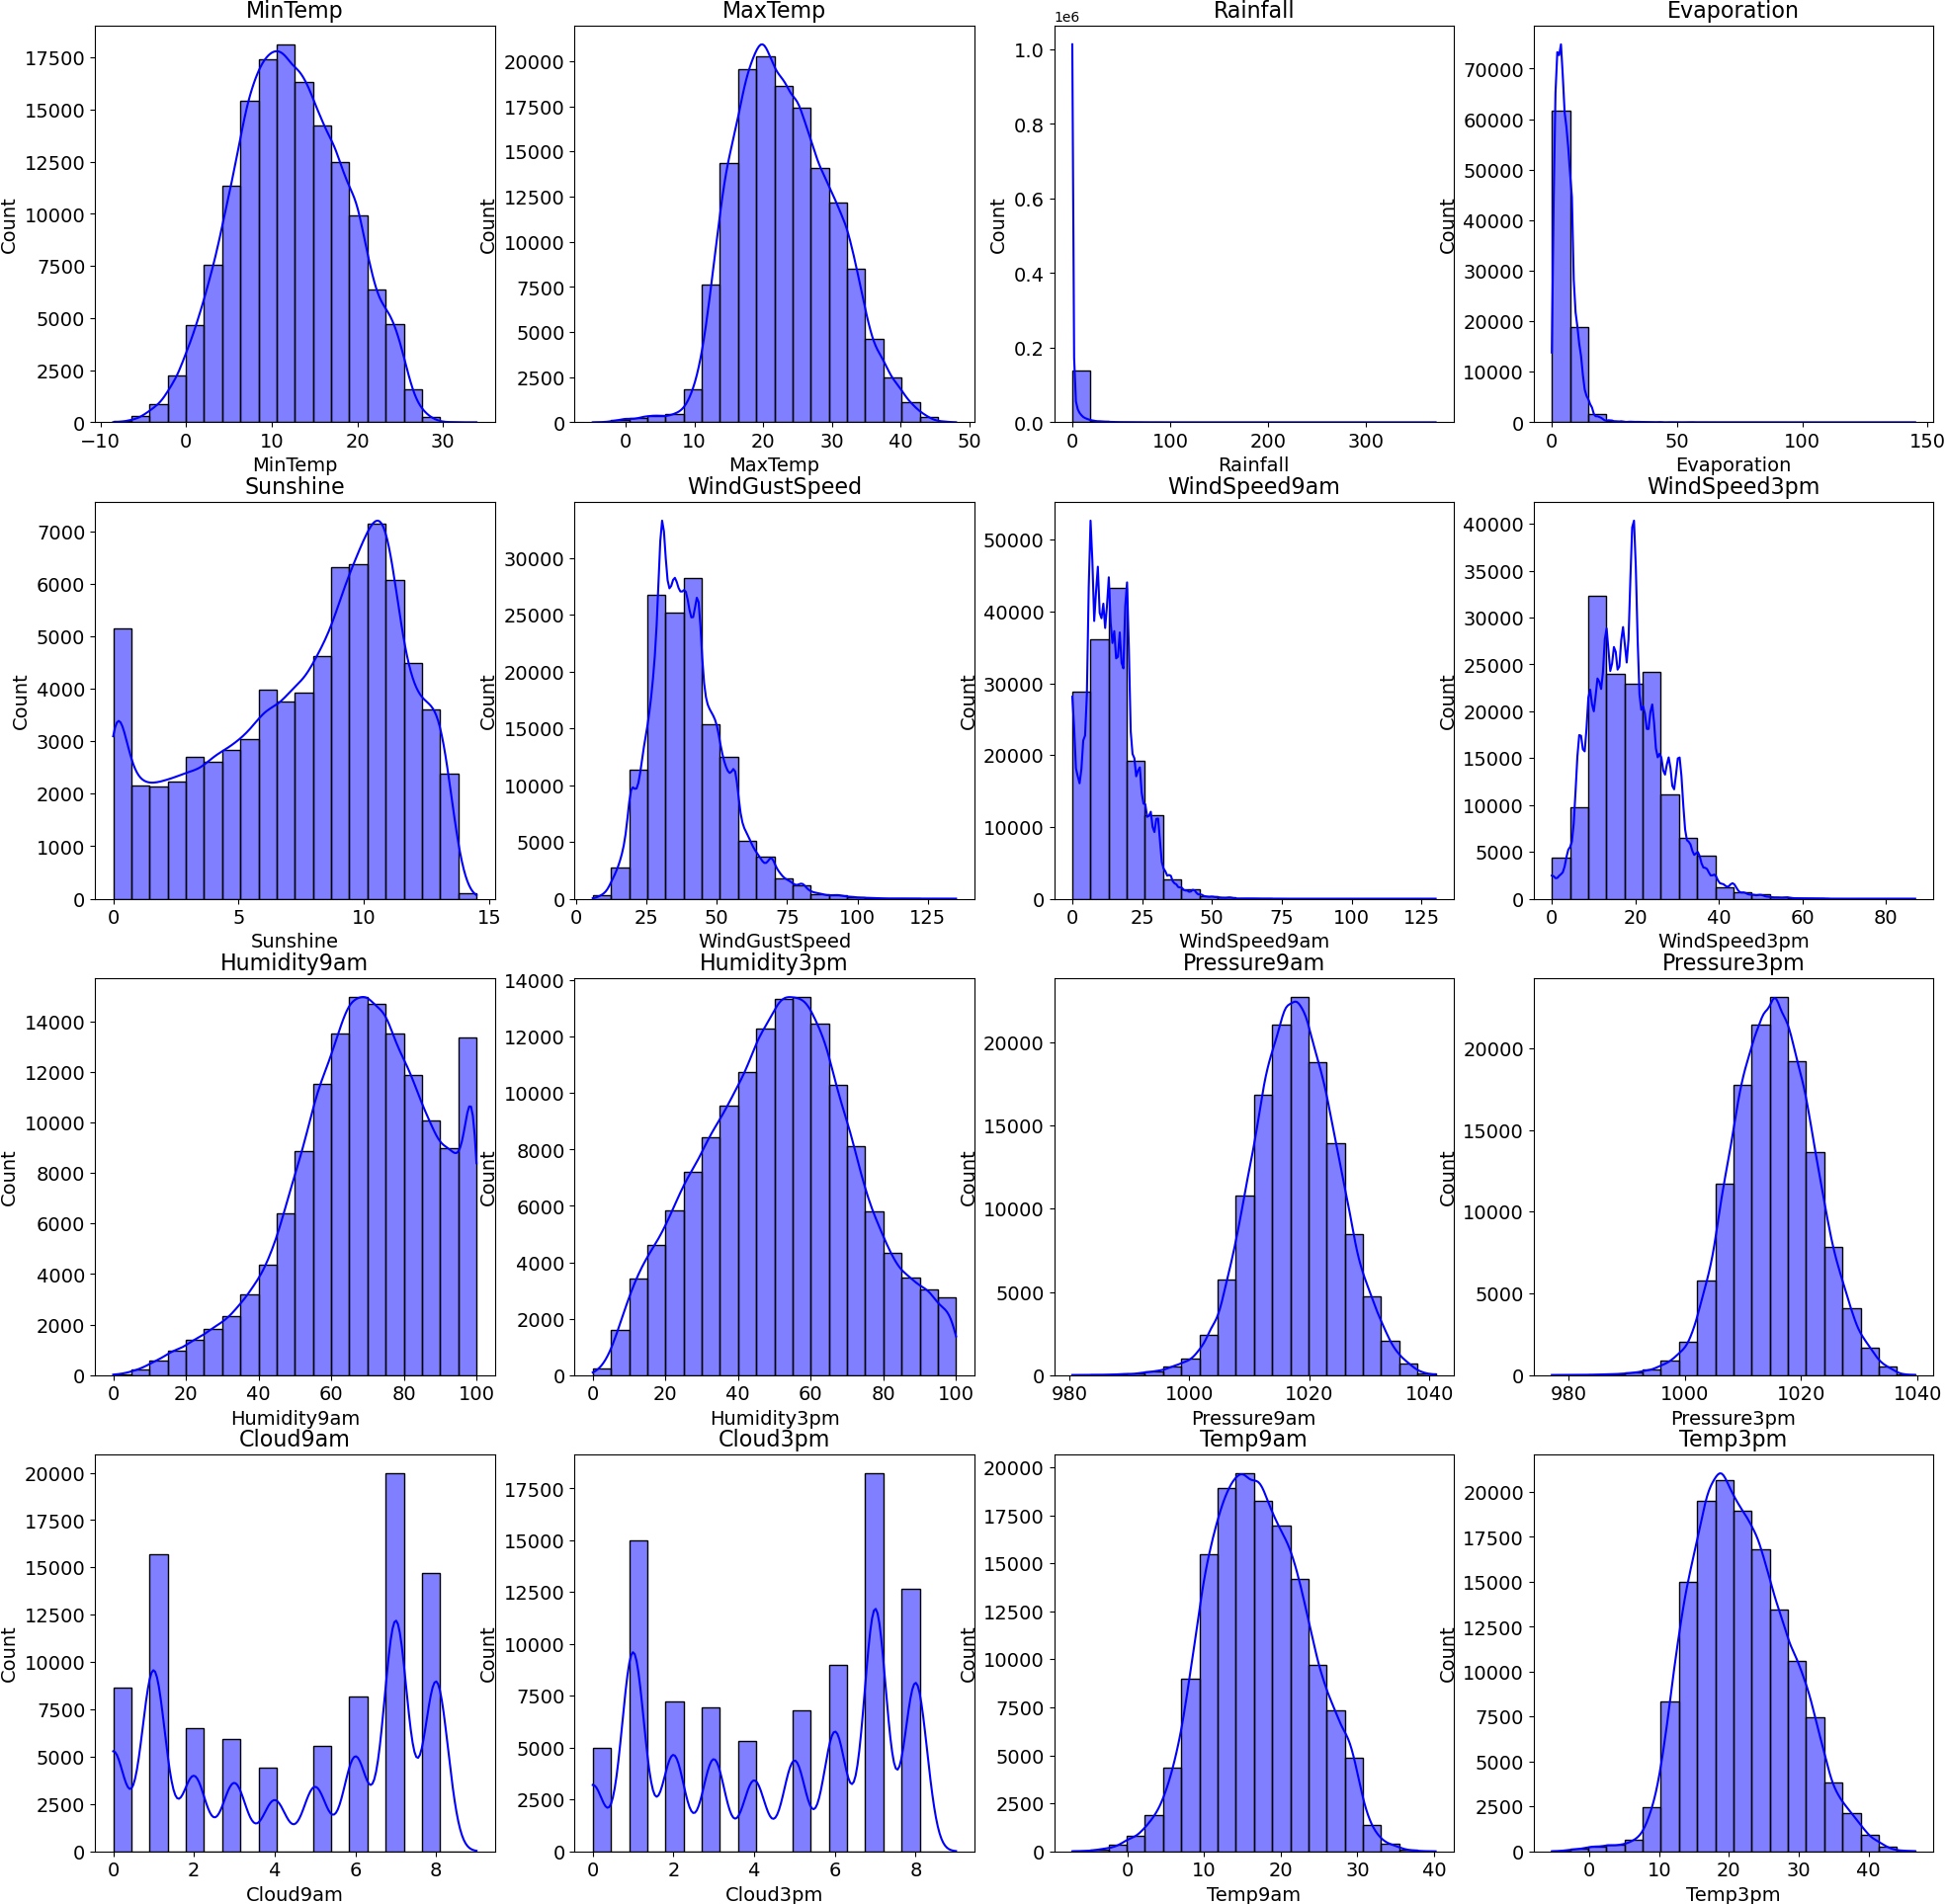
\includegraphics[width=460px]{EDA/histograms.png}%
\caption{Histograms of Numerical columns}%
\end{figure}

%
\newpage%
\subsection{Bar Charts of Categorical columns}%
\label{subsec:BarChartsofCategoricalcolumns}%


\begin{figure}[h!]%
\centering%
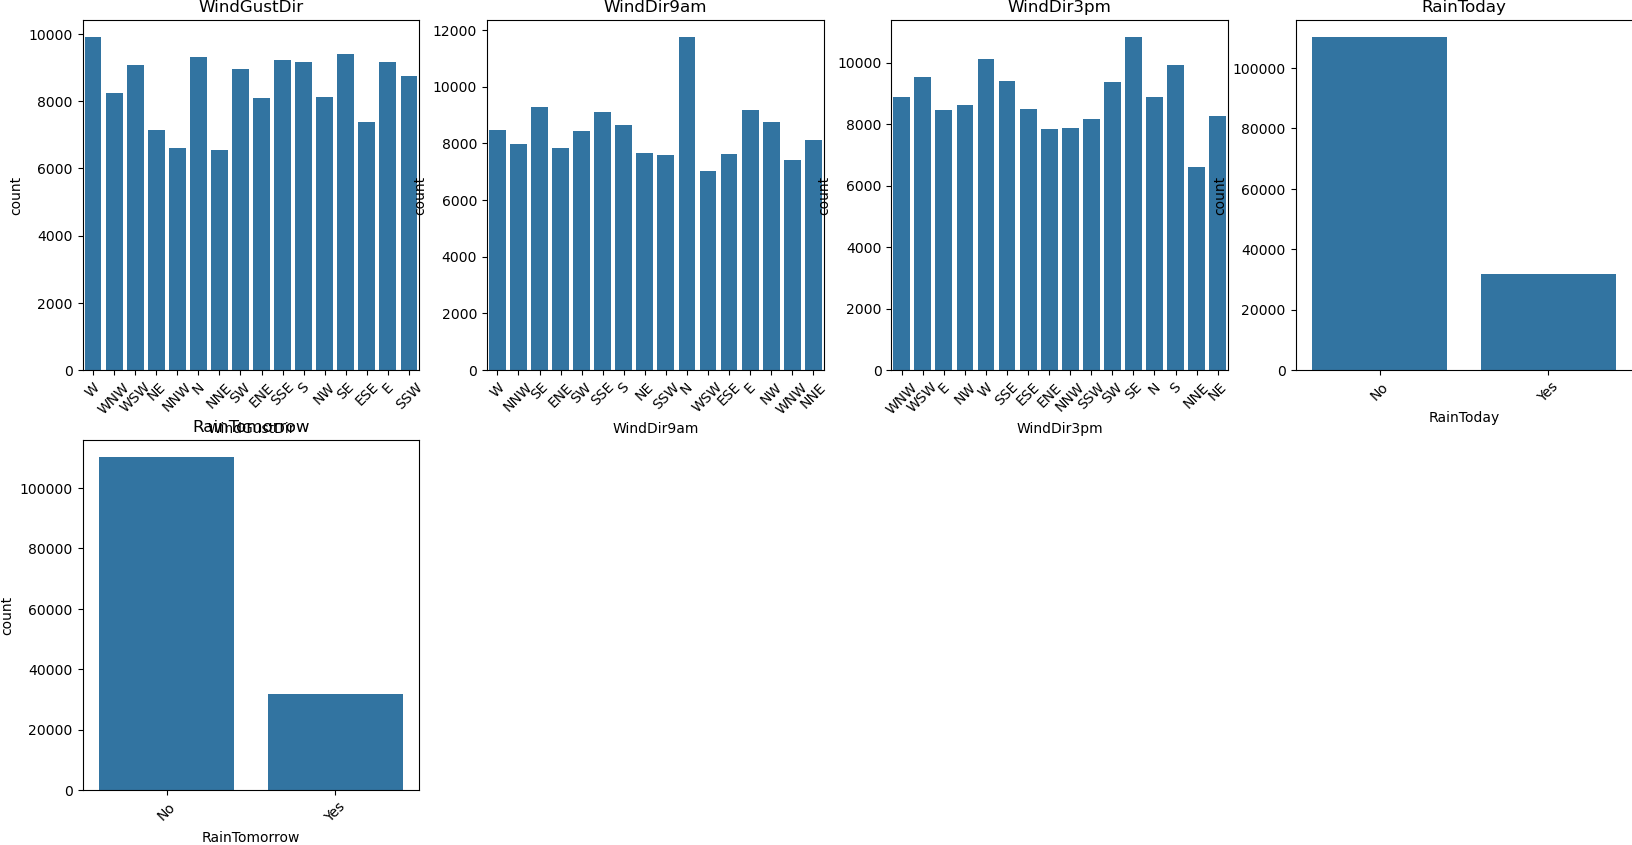
\includegraphics[width=460px]{EDA/bar_charts.png}%
\caption{Bar Charts of Categorical columns}%
\end{figure}

%
\end{document}